%Document FORMATTING [D]
\documentclass[12pt]{article}
\usepackage[utf8]{inputenc}
\usepackage[top=2.5cm,bottom=2cm,right=4cm, left=4cm,includefoot]{geometry}
\usepackage{rotating}
\usepackage{tikz}
\usepackage{booktabs}
%BIBLIOGRAPHY
\usepackage[hyphens]{url}
\urlstyle{same}

\usepackage{booktabs}
\usepackage{lipsum}
\usepackage{setspace}
\usepackage{amsmath}

\usepackage{tabularx}
\usepackage{array}
\usepackage{floatrow} %forces table caption to top
\floatsetup[table]{capposition=top}
\usepackage{booktabs}

\usepackage{graphicx} %for figures
\graphicspath{ {./images/} } % put images in this directory
\usepackage{caption}
\captionsetup{margin=10pt,font=small} 
\usepackage{subcaption}

\usepackage{enumitem}
\newenvironment{QandA}{\begin{enumerate}[label=\bfseries\alph*.]\bfseries}
                      {\end{enumerate}}
\newenvironment{answered}{\par\normalfont}{}
\usepackage{lipsum}

\usepackage{array}
\newcolumntype{L}[1]{>{\raggedright\let\newline\\\arraybackslash\hspace{4pt}}m{#1}}
\newcolumntype{C}[1]{>{\centering\let\newline\\\arraybackslash\hspace{4pt}}m{#1}}
\newcolumntype{R}[1]{>{\raggedleft\let\newline\\\arraybackslash\hspace{4pt}}m{#1}}
\usepackage{floatrow}
% Table float box with bottom caption, box width adjusted to content
\newfloatcommand{capbtabbox}{table}[][\FBwidth]
\usepackage{lastpage}   
\usepackage{fancyhdr}
\pagestyle{fancy}
\fancyhead{}        %clears fancy head
\fancyfoot{}        %clears fancy foot
\cfoot{\makebox[\textwidth][c]{\thepage\ of \pageref{LastPage}}}
\renewcommand{\headrulewidth}{0pt}
\usepackage{titlesec}
\titleformat*{\section}{\large\bfseries}
\titleformat*{\subsection}{\bfseries}

\usepackage{pdfpages}

\begin{document}

% Title Page:
% Title: Initial Report of Group <Group ID>
% Name of project
% List of team members with their a-numbers

\begin{titlepage}
    \begin{center}
        \vspace*{100pt}
        \large{Faculty of Engineering, Computer\\ and Mathematical Sciences}\\
        \vspace*{15pt}
  
        {\large SIVT 1}\\
        [-5pt]
        \line(1,0){350}\\
        [15pt]
        {\huge \bfseries Initial Report }\\
        [1pt]
        \line(1,0){350}\\
        [5pt]
        {\large \bfseries Software Engineering \& Project}
        \\
        [10pt]
        {\Large 2020}\\
        \vspace*{45pt}
        \textsc{\normalsize Members:}\\
        [10pt]
    \centering
    \begin{minipage}{ .45\textwidth}
        \centering
        {\normalsize 
        \flushleft Gabriel P.C.L De Almeida
         \flushleft Jackson Dearing 
         \flushleft Rhett Hull
        \flushleft Steve Monger 
       \flushleft Kristina Plavsa
       \flushleft Colin Ross
       \flushleft Joshua Tatton
       \flushleft Elliot Wheatland
       \flushleft Brian Yip\\}
    \end{minipage}%
    \begin{minipage}{0.45\textwidth}
        \centering
        {\normalsize 
        \flushright a1673698
        \flushright a1686411
        \flushright a1706579
        \flushright a1176574
        \flushright a1723663
        \flushright a1704822
        \flushright a1690417
        \flushright a1717968
        \flushright a1751117\\}
    
    \end{minipage}\\
    
    \vspace*{20pt}
        \textsc{\normalsize Submitted on:}\\
        [5pt]
        {$18^{th}$ August 2020}\\
    \end{center}
\end{titlepage}
%______________________________________
\cleardoublepage
\newgeometry{margin=2.54cm,left=2.0cm,right=2.0cm, includefoot}
%_______________________________________

% Project Vision:
% Brief (100-200 words) summary of the project vision in your own words
%%COMPLETE & REVIEWED BY KP
\section{Project Vision}
\begin{spacing}{1.3}
% I have added more backround and just trimmed the wording - KP
Propic is a company that provides analyst services for the Real Estate sector, using big data and artificial intelligence. Their business intelligence product, ReVeal AI, generates recommendations for real estate agents for listings and appraisals. Part of this development process involves analysts querying the system to facilitate answering business questions. The transformation process has been refined over time in order to facilitate answering increasingly sophisticated and abstract business questions. These refinements have introduced increased complexity, leading to difficulty in understanding, validating and risk-managing the transformation process. 

The aim of the project is to provide a visualisation tool which allows analysts to easily understand the data transformation. For each SQL script provided by a user, this tool will derive the relevant table and data lineage. The information will be displayed in a web browser in a clear and intuitive manner. Interactive elements will allow users to highlight only the data lineage information which is related to an individual table. This will enable developers and the end user to better understand why, how and where recommendations are coming from. This will enable Propic to better refine their understanding and build more reliable and explanable systems.
\end{spacing}


% Customer Q&A:
% This section should summarise the questions you asked during the kickoff meeting and the client's responses. You should starting writing down potential questions as soon as you got assigned to a team and project
% This section should also contain a brief (100-200 words) reflection on how the kickoff meeting went, what you could have done differently, and what you've learned for the next meeting, maybe including potential follow-up questions

\section{Customer Q\&A}
\begin{spacing}{1.3}
The first customer Q\&A was a general overview of the final product with the product owner and provided. The meeting provided the necessary starting information to begin the first sprint. The product owner described their final product as being a web application that allows developers and analysts to input a presto SQL file, from which an interactive data lineage will be visualized. For example, given an SQL script, it will be possible to trace the source and transformation of a column of data from a "Users" table with ease. \\ \vspace{-5pt}

The following questions were asked during the kickoff meeting:
\begin{QandA}
   \item What is the domain of the provided input? (Aside from being SQL queries) Is there any other formal specification you have already?
        \begin{answered}
            The file input will be a SQL presto file.
        \end{answered}

   \item What user action triggers the visualisation?
         \begin{answered}
            The output is automatically a visual representation, i.e. given an SQL file path, it should automatically load the visualization, without running other scripts.
         \end{answered}
         
    \item Do you have a preference or disposition to any specific subset of available tools, programming languages or frameworks. If so, what are they?
        \begin{answered}
            No restrictions, open source is acceptable. Input scripts must be be Presto syntax.
        \end{answered}
        
    \item Do you have a preference for the application to be available in the web browser or as a native application? If the latter, what operating system do Propic developers use?
        \begin{answered}
            Please use a system agnostic solution, such as a web application.
        \end{answered}
\end{QandA}

For the first sprint, the Product Owner recommended the development team focus on parsing the Presto SQL code. The first sprint iteration of the product should thus output a table of data showing which tables are using which data. As demonstrated in Section~\ref{sec:snapshot}, the first sprint is dedicated to initial configuration of the system, as well as achieving this initial goal. \\
\vspace{-5pt}

On reflection, the team determined the initial meeting was successful, as sufficient information was gathered to understand the Product Owner's vision, and the core objectives that we must achieve. All group members engaged with the product owner, asking insightful follow-up questions and collectively created a list of tasks and objectives. \\ \vspace{-5pt}

However, the team determined that the scrum master should take primary lead during meetings as the primary spokesperson and chairman, to ease communication with a large development team. In particular, the scrum master should have been the person posing the questions formulated by the team, and delegating speaking responsibilities to other members in the group. This would have facilitated in-depth discussions with the product owner about their needs and allowed for everyone the chance to provide their input and pose relevant follow-up questions. \\

In hindsight, follow-up questions were posed to the client after internal discussions, which were as follows:
\begin{QandA}
    \item Who is the typical intended user of our tool? What kind of typical technical background do they come from? Are the staff low-level analysts or high-level management for example?
    \begin{answered}
        Users will be data analysts and data engineers whose role requires an in-depth understanding and frequent interaction of the data pipeline.
    \end{answered}
    
    \item How is this tool going to assist and be integrated into their workflow?
    \begin{answered}
        It is going to be used in the maintenance of ETL (Extract, transform and Load Data) development process. This will be useful to see the complete data flow from origin to destination. The main goal is to provide a better understanding to the user of what happened to the data throughout the life cycle.
    \end{answered}
    
    \item Can you confirm that a Web-based application is suitable for Propic?
    \begin{answered}
        Yes, a Web-based application is suitable. To make the deployment easier for us, I would prefer using technology like Docker. But I am no expert on it, happy to see what you recommend.
    \end{answered}
\end{QandA}

\end{spacing}

% Users:
% Describe the roles you identified after the kickoff meeting (roles in the sense of different kinds of users of your app)
% You should list the roles and provide brief summaries of their responsibilities and potential actions (3-4 sentences)

\section{Users}
\begin{spacing}{1.3}
The users identified by the development team after the kickoff meeting are Data Analysts and Developers. 

\paragraph{Data Analysts:}
Typically, data analysts have a mathematical background with some software and computer science knowledge and experience. Propic data analysts are responsible for querying the system, and determining how the data was transformed, why the data was transformed and leveraging this knowledge to provide Real-Estate recommendations. The analyst shall be able to use the data visualisation tool to quickly identify the data lineage and its relations by inputting their necessary scripts. They will then be able to interact with the tool to further explore the relationships.

\paragraph{Developers:}
Similar to data analysts, developers have some mathematical background, although they have much more experience in the field of computer science. Propic developers develop and maintain the code and database queries for the tool. Mapping the lineage in an interactive way will provide them with a reliable method of validating and maintaining the extract, transform, and load process and reduce the time needed to analyse and understand the scripts. 


\end{spacing}

% Software Architecture:
% Rough sketch of the potential architecture of your application
% Can be structured UML, but can also be an ad hoc boxes-and-arrows diagrams with a legend
% Provide a brief (100-200 words) justification for the architecture you chose
%214 words 
%Reviewed by KP

\section{Software Architecture}
\begin{spacing}{1.3}

\begin{figure}[h!]
  \caption{Application Architecture Schematic}
  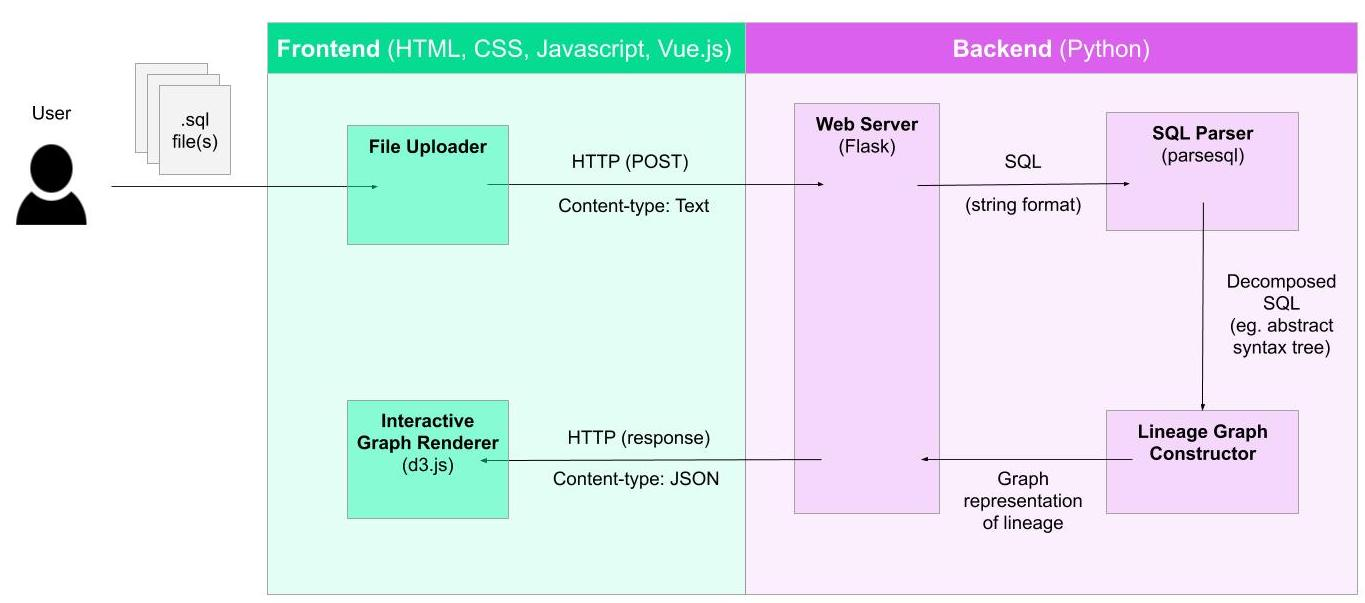
\includegraphics[width=\textwidth]{architecture.jpg}
  \label{fig:software-architecture-schematic}
\end{figure}

The architecture for the application seen in Figure \ref{fig:software-architecture-schematic} represents a Client-Server web application. A web application was selected based on the following considerations:

\begin{itemize}
\item Existence of relevant, open-source data visualisation libraries in JavaScript
\item Ability to implement back-end logic in Python (aligning with team member skills)
\item Maximise applications' availability - running through the web browser makes it independent of any particular operating system
\end{itemize}

The Client-Server model allows for separation of the SQL analysis logic from the visualisation components. This separation facilitates incremental development and increases modularity which is ideal for large, collaborative projects.\newline

For the average application usage, a user shall upload an sql file as input to the front-end File Uploader which will upload and convert the file content to string format. The file content shall be sent via HTTP POST to the Web Server which will forward the SQL content to a dedicated SQL Parser. In the back-end, the SQL Parser and Lineage Graph Constructor are responsible for decomposing the SQL input and formulating a programmatic representation of a graph containing the lineage relationships. This graph of lineage information shall be sent back to the front end in JSON format. The Interactive Graph Renderer shall take the lineage information and produce an interactive visual in the web browser. 
\end{spacing}

% Tech Stack and Standards:
% List the likely tech stack for your application (distinguish between back-end and front-end, programming languages and frameworks)
% Agree on tools for communication and development (e.g., Slack, IDEs, etc.)
% Agree on coding standards
% Provide justifications for your choices

\section{Tech Stack and Standards}
\begin{spacing}{1.3}

\subsection{Team Communications}
\paragraph{Technologies Considered:}
Slack, Facebook Messenger, Email, Discord

\paragraph{Decision Criteria:}
\begin{itemize}
\item Instant messaging
\item Multiple text channels
\item Voice channel support
\item GitHub integration
\item Currently used services
\end{itemize}

\paragraph{Chosen:}
Discord

\paragraph{Justification:}
Slack and Discord rated highest for instant messaging, text channel support and reliable voice channel service. Despite Slack having better integration capabilities with GitHub, Discord was chosen as it was already regularly used by team members. Adoption of yet another communication service may have over-saturated the communication space for team members and been detrimental to responsiveness.

\subsection{Version Control and Remote Repository}
\paragraph{Chosen:}git with GitHub
\paragraph{Justification:}
Using git for version control and GitHub to host the remote repository was mandated for the project. This also extended to the use of GitHub Projects for project planning operations including issue tracking and sprint planning.

\subsection{Front-End Technologies}
\paragraph{Technologies Considered:}
Vue.js, Angular, React

\paragraph{Decision Criteria:}
\begin{itemize}
\item Learning curve
\item Development team experience
\item Flexibility
\item Scalability
\item Performance
\item Size
\end{itemize}

\paragraph{Chosen:} Vue.js
\paragraph{Justification:} In order to navigate the numerous criteria, a data-driven approach was taken by constructing a decision matrix seen in Table 1 which resulted in Vue.js being the most optimal front end framework. Vue is a light-weight JavaScript library used to develop interactive web interfaces. It has extensive and excellent documentation that makes the front-end development a smooth process for developers of all levels. One of Vues' features is its loosely coupled components, which allows the development team to create custom elements and re-use them later if needed. It also allows for imports of existing components from external sources, therefore decreasing development time. An important library that will be used in the front-end for http communication is called Axios.

\begin{table}[htbp!]
\centering
\small
\caption{Front-end Framework Decision Matrix}
\label{my-label}
\begin{spacing}{1.1}
\resizebox{0.8\textwidth}{!}{
\begin{tabular}{@{}rc|c|c|c|c|c|c@{}}
\hline
\toprule

&&\multicolumn{6}{c}{\bfseries\footnotesize Options}\\ \hline

\bfseries{\footnotesize Criteria} 
&\bfseries{\footnotesize Weight} 
&\multicolumn{2}{c|}{\bfseries\footnotesize Angular}
&\multicolumn{2}{c|}{\bfseries\footnotesize React}
&\multicolumn{2}{c}{\bfseries\footnotesize Vue}\\ \hline
 & & {\footnotesize Score}&
 {\footnotesize Total}&
 {\footnotesize Score}&
 {\footnotesize Total}&
 {\footnotesize Score}&
 {\footnotesize Total} \\\hline
 
Learning Curve  & 6 & 3 & 18 & 4 & 24 & 5 & 30\\
DT Experience   & 6 & 3 & 18 & 2 & 12 & 5 & 30 \\
Flexibility     & 5 & 2 & 10 & 6 & 30 & 6 & 30\\
Scalability     & 4 & 6 & 24 & 5 & 20 & 2 & 8\\
Performance     & 4 & 5 & 20 & 6 & 24 & 6 & 24\\ 
Size            & 2 & 3 & 6 & 2 & 4 & 6 & 12\\\hline

& Total &\multicolumn{2}{c|}{\bfseries\footnotesize 98}& \multicolumn{2}{c|}{\bfseries\footnotesize 114} &  \multicolumn{2}{c}{\bfseries\footnotesize 134}\\

\bottomrule
\end{tabular}}
\end{spacing}{}
\end{table}

\subsection{Back-End Technologies}

\paragraph{Technologies Considered:} Python with either Flask or Django, Javascript with Express.js or Node.js

\paragraph{Decision Criteria:}
\begin{itemize}
\item Ease of Use
\item Development team experience
\item Simplicity
\item Compatibility with Front End Technology
\item Size
\end{itemize}
\paragraph{Chosen:} Python, Flask
\paragraph{Justification:}
The use of Python as the back-end language of choice was heavily influenced by the development teams' collective aggregate experience with Python. As shown in Figure \ref{fig:lang-experience}, Python is one of the most commonly known languages amongst the team. Coupled with the fact that Python has a shallow learning curve in comparison to other languages, makes it the language of choice for back-end technology. The library chosen to be used with python is Flask. Flask excels as a lightweight back-end for simple web applications, whereas Django has a large number of features that are unlikely to be used for the project. This makes Flask an ideal choice for the scope of this project. These choices are summarized in the decision matrix shown in Table 2. \ref{fig:backend_mat}.

%It is noted that as well as pure applicability to the problem, the collective expertise of the team was also an important factor when determining a tech stack. For reference of this, Figure \ref{fig:lang-experience} provides a guide for the aggregate language specific skills of the team prior to commencing the project.

\begin{figure}[!h]
  \caption{Development Team Language Experience}
  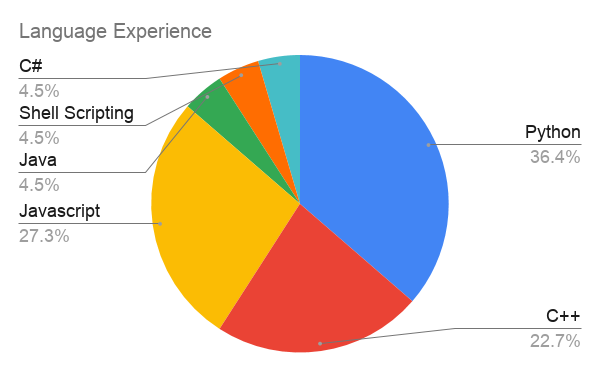
\includegraphics[width=\textwidth]{images/lang-experience.png}
  \label{fig:lang-experience}
\end{figure}

\begin{table}[htbp!]
\centering
\small
\caption{Backend Technology Decision Matrix}
\label{my-label}
\begin{spacing}{1.1}
\resizebox{\textwidth}{!}{
\begin{tabular}{@{}r c|c|c|c|c|c|c|c|c@{}}
\hline
\toprule

&
&\multicolumn{4}{c|}{\bfseries\footnotesize Python}
&\multicolumn{4}{c}{\bfseries\footnotesize Javascript}\\ \hline

\bfseries{\footnotesize Criteria} 
&\bfseries{\footnotesize Weight} 
&\multicolumn{2}{c|}{\bfseries\footnotesize Flask}
&\multicolumn{2}{c|}{\bfseries\footnotesize Django}
&\multicolumn{2}{c|}{\bfseries\footnotesize Express.js}
&\multicolumn{2}{c}{\bfseries\footnotesize Node.js}\\ \hline

     &  & {\footnotesize Score}&
     {\footnotesize Total}&
     {\footnotesize Score}&
     {\footnotesize Total}&
     {\footnotesize Score}&
     {\footnotesize Total}&
     {\footnotesize Score}&
     {\footnotesize Total}   \\\hline


Ease of Use     & 6 & 6 & 36 & 6 & 36 & 4 & 24 & 4 & 24   \\
DT Experience   & 6 & 6 & 36 & 6 & 36 & 4 & 24 & 4 & 24   \\
Simplicity      & 5 & 4 & 20 & 5 & 25 & 5 & 25 & 5 & 25   \\
Size            & 4 & 6 & 24 & 4 & 16 & 6 & 24 & 5 & 20   \\
Compatability*      & 6 & 6 & 36 & 5 & 30 & 6 & 36 & 6 & 36   \\ \hline
& Total &\multicolumn{2}{c|}{\bfseries\footnotesize 152}& \multicolumn{2}{c|}{\bfseries\footnotesize 143} &  \multicolumn{2}{c|}{\bfseries\footnotesize 133} &  \multicolumn{2}{c}{\bfseries\footnotesize 129}   \\

\bottomrule
\end{tabular}}
\end{spacing}{}
\end{table}

\subsection{Coding Standards}
Although Propic does not require the adoption of any specific technology or standard, the development team agreed that it would be good practice to still enforce coding standards to optimise consistency, readability and maintainability. Given the tech stack decisions, this was predominantly relevant to Python code (back-end) and JavaScript code (front-end). For these, the PEP style guidelines will be used for python with a small addition for function commenting (available on the project wiki) as well as the Airbnb JavaScript style guide which will be assisted with static analysis by ESLint.

\subsection{Integrated Development Environment}
\paragraph{Technologies Considered:}
VSCode, PyCharm, Jupiter Notebook, Vim, Atom, Sublime
\paragraph{Decision Criteria:}
\begin{itemize}
\item Compatibility for languages and frameworks to be used
\item Static analysis extensions (specifically for PEP and Airbnb style guides)
\item Development team experience and preference
\item Version control integration
\end{itemize}

\paragraph{Chosen:}
VSCode (preferred guideline)

\paragraph{Justification:}
Given the above decisions on languages, frameworks and coding standards, it was decided that the preferred IDE for development will be VSCode. This is because it is free, straightforward to use and has good support for Python as well as JavaScript in terms of syntax highlighting and extensions for static analysis. It is also extremely versatile with a rich library of extensions which make it highly customisable. The universal use of a VSCode throughout the team is not being mandated as a range of other IDEs can also be configured in accordance with the projects' style preferences. This allows any developer to use their own favourite IDE, if preferred.
\end{spacing}

% Group Meetings and Team Member Roles:
% How frequently and for how long do you intend to (virtually) meet?
% Please remember to time-box the meetings!
% When will you schedule the sprint retrospective meetings?
% Did you arrange for additional feedback channels with the customer (e.g., via Slack or email)?
% Please name the Scrum Masters for each sprint (each team member can only be the Scrum Master for up to one sprint)
\begin{spacing}{1.3}

\section{Group Meetings and Team Member Roles}

Stand-up meetings are currently scheduled for two meetings per week. These are to be held every Monday and Friday until the completion of the project. During the later stages of the project, once the team has settled into their roles, a third stand-up meeting may be added. These stand-up meetings are time-boxed to 15 minutes. This ensures that there is sufficient time for all team members to share their progress, intended work and blockers, whilst keeping the meeting short. Should any problems arise during the stand-up meetings, individual team members may schedule `offline' meetings to work through potential solutions. \\
\vspace{-5pt}

Client meetings, including the Sprint review and planning meetings, will be held with the tutor bi-weekly on Fridays at 1pm. The review and planning meetings will be combined to a single meeting due to the availability of contact time with the tutor (and client). This single meeting will be time-boxed to 25 minutes. \\
\vspace{-5pt}

Sprint retrospectives are usually held between the sprint review and sprint planning meetings, however due to the nature of the single review-planning meeting, this will be held at a separate time. 
This retrospective meeting will be held after the review-planning in place of the `daily' stand-up.

\subsection{Scrum Masters}

The scrum masters for each sprint are listed in Table \ref{tab:scrumMasters}.
Scrum masters were selected through self-nomination and election and assigned at random to sprints. 

\begin{table}[htbp]
    \centering
    \begin{tabular}{@{}r|l@{}}
    \toprule
        \textbf{Sprint} & \textbf{Scrum Master} \\
        \hline
        1 & Colin Ross \\
        2 & Jackson Dearing\\
        3 & Joshua Tatton\\
        4 & Elliot Wheatland\\
        5 & Steven Monger\\
        \bottomrule
    \end{tabular}
    \caption{Scrum Masters}
    \label{tab:scrumMasters}
\end{table}

\end{spacing}

% Snapshot:
% Provide a snapshot before first sprint (see snapshot assignment)

\section{Snapshot}
\label{sec:snapshot}
See pages 11 - 14.
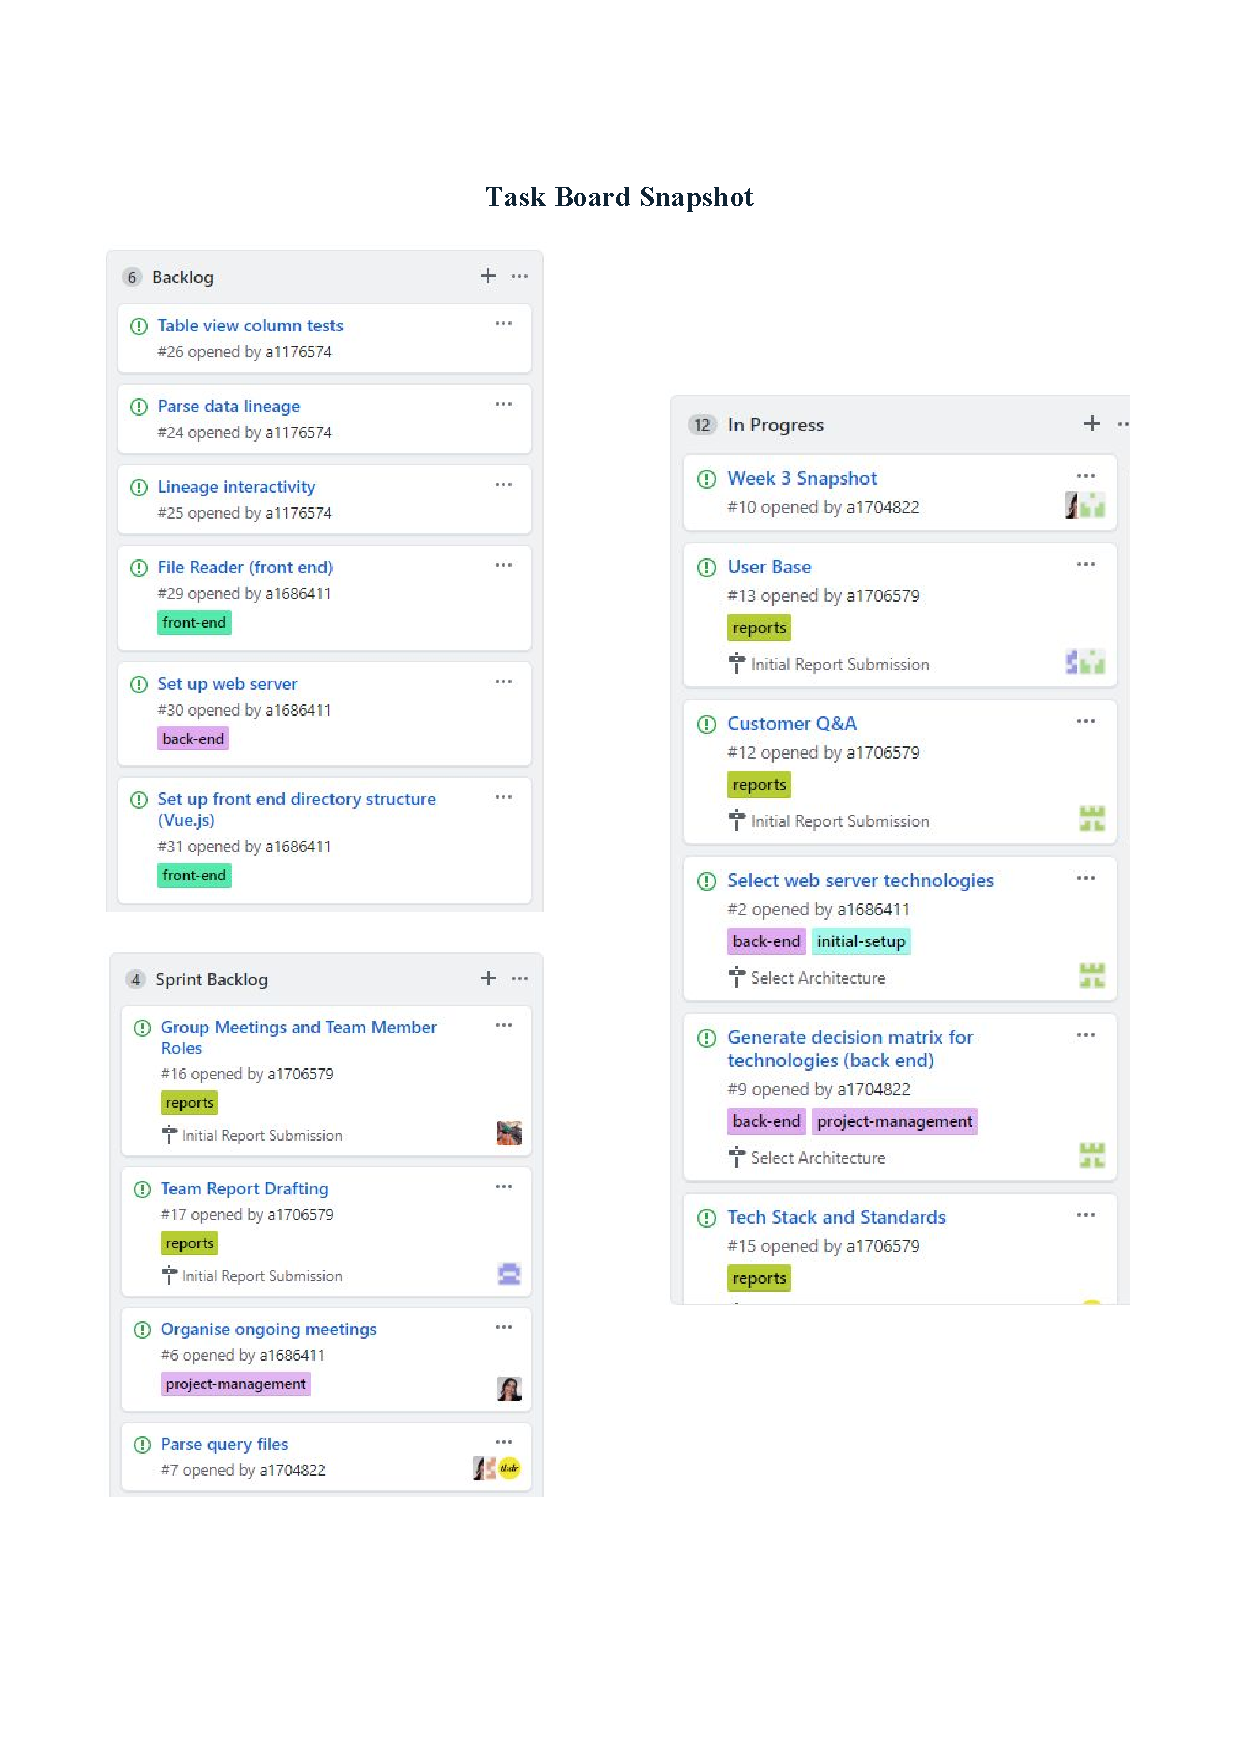
\includepdf[pages=-, pagecommand={\thispagestyle{fancy}},]{snapshot_week03_SIVT1.pdf}

\end{document}
